% -*- latex -*-
%%%%%%%%%%%%%%%%%%%%%%%%%%%%%%%%%%%%%%%%%%%%%%%%%%%%%%%%%%%%%%%%
%%%%%%%%%%%%%%%%%%%%%%%%%%%%%%%%%%%%%%%%%%%%%%%%%%%%%%%%%%%%%%%%
%%%%
%%%% This text file is part of the source of 
%%%% 'Parallel techniques'
%%%% by Ángel de Vicente, copyright 2019
%%%%
%%%% TO DO:
%%%%
%%%% barnes-hut.tex : description of the Barnes-Hut algorithm
%%%%
%%%%%%%%%%%%%%%%%%%%%%%%%%%%%%%%%%%%%%%%%%%%%%%%%%%%%%%%%%%%%%%%
%%%%%%%%%%%%%%%%%%%%%%%%%%%%%%%%%%%%%%%%%%%%%%%%%%%%%%%%%%%%%%%%

\emph{The material in this chapter is an abriged version of the
  \url{https://people.eecs.berkeley.edu/~demmel/cs267/lecture26/lecture26.html} webpage}

\Level 0 {Introduction}
\label{sec:bh-intro}

Far field forces like gravity are very expensive to compute because the force on
each particle depends on all the other particles, as we saw in the naïve
solution to the n-body problem \ref{sol_ex:basic-nbody}.

\begin{verbatim}
a = 0.0
DO i = 1,n
   DO j = i+1,n
      rji = r(j,:) - r(i,:)
      r2 = SUM(rji**2)
      r3 = r2 * SQRT(r2)
      a(i,:) = a(i,:) + m(j) * rji / r3
      a(j,:) = a(j,:) - m(i) * rji / r3
   END DO
END DO
\end{verbatim}

Thus, the calculation cost rises as O(n2), so even with parallelism, the far
field forces will extremely expensive to compute. Fortunately, it turns out that
there are clever divide-and-conquer algorithms which only take O(n log n) or
even just O(n) time for this problem.

\Level 0 {How to reduce the number of particles in the force sum}
\label{sec:bh-reduce-number-particles}

Suppose we wanted to compute the gravitational force on the earth from the known
stars and planets. A glance skyward on a clear night reveals a dauntingly large
number of stars that must be included in the calculation, each one contributing
a term to the force sum.

One of those dots of light we might want to include in our sum is, however, not
a single star (particle) at all, but rather the Andromeda galaxy, which itself
consist of billions of stars. But these appear so close together at this
distance that they show up as a single dot to the naked eye. It is tempting --
and correct -- to suspect that it is good enough to treat the Andromeda galaxy
as a single point anyway, located at the center of mass of the Andromeda galaxy,
and with a mass equal to the total mass of the Andromeda galaxy. This is
indicated below, with a red x marking the center of mass. More mathematically,
since the ratio

\begin{verbatim}
         size of box containing Andromeda
D/r  = -------------------------------------
       distance of center of mass from Earth
\end{verbatim}

is so small, we can safely and accurately replace the sum over all stars in
Andromeda with one term at their center of mass (see figure \ref{fig:bh-Andromeda}).

\begin{figure}[!htbp]
  \centering
  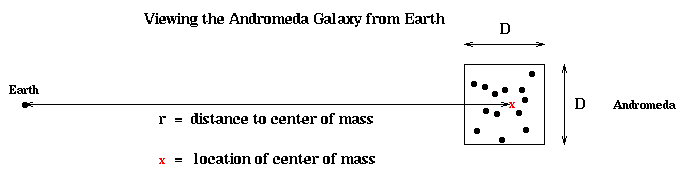
\includegraphics[width=0.9\textwidth]{graphics/bh/Andromeda.png}
  \label{fig:bh-Andromeda}
  \caption{Viewing the Andromeda Galaxy from Earth}
\end{figure}

This idea is hardly new, but what is new is applying this idea
recursively. First, it is clear that from the point of view of an observer in
the Andromeda galaxy, our own Milky Way galaxy can also be well approximated by
a point mass at our center of mass. But more importantly, within the Andromeda
(or Milky Way) galaxy itself, this geometric picture repeats itself as shown
below: as long as the ratio D1/r1 is also small, the stars inside the smaller
box can be replaced by their center of mass in order to compute the
gravitational force on, say, the planet Vulcan. This nesting of boxes within
boxes can be repeated recursively (see figure \ref{fig:bh-Andromeda1})
\begin{figure}[!htbp]
  \centering
  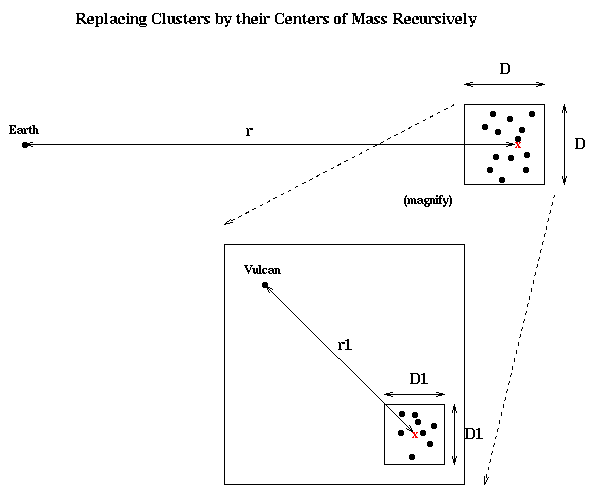
\includegraphics[width=0.8\textwidth]{graphics/bh/Andromeda1.png}
  \label{fig:bh-Andromeda1}
  \caption{Replacing Clusters by their Centers of Mass Recursively}
\end{figure}

\Level 0 {Quadtrees and Octtrees}
\label{sec:bh-trees}

What we need is a data structure to subdivide space that makes this recursion
easy. The answer in 3D is the octtree, and in 2D the answer is the quadtree. We
begin by describing the quadtree, because it is easier to draw in 2D; the
octtree will be analogous. The quadtree begins with a square in the plane; this
is the root of the quadtree. This large square can be broken into four smaller
squares of half the perimeter and a quarter the area each; these are the four
children of the root. Each child can in turn be broken into 4 subsquares to get
its children, and so on. This is shown below. Each colored dot in the tree
corresponds to a square in the picture on the left, with edges of that color
(and of colors from higher tree levels). See figure \ref{fig:bh-Quadtree1}.

\begin{figure}[!htbp]
  \centering
  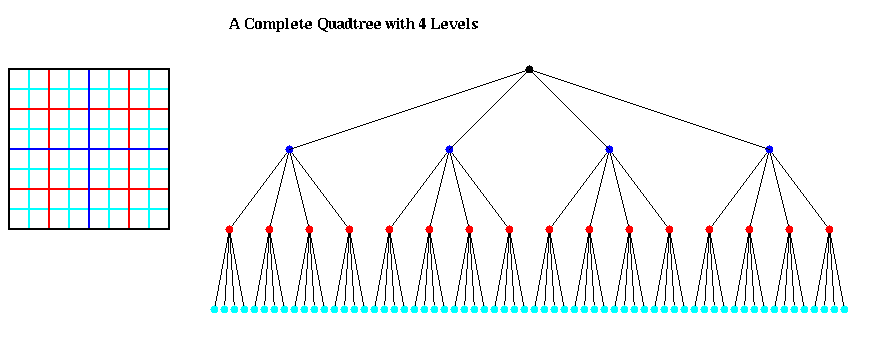
\includegraphics[width=0.9\textwidth]{graphics/bh/Quadtree1.png}
  \label{fig:bh-Quadtree1}
  \caption{A complete quadtree with 4 levels}
\end{figure}

An octtree is similar, but with 8 children per node, corresponding to the 8
subcubes of the larger cube, as illustrated in figure \ref{fig:bh-Octtree}.

\begin{figure}[!htbp]
  \centering
  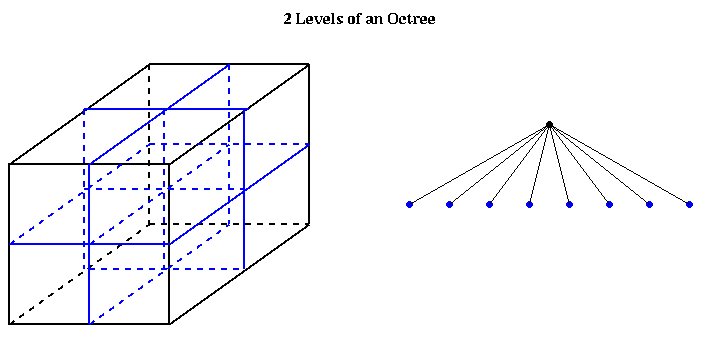
\includegraphics[width=0.9\textwidth]{graphics/bh/Octtree.png}
  \label{fig:bh-Octtree}
  \caption{2 Levels of an Octtree}
\end{figure}


The algorithm we present below begins by constructing a quadtree (or octtree) to
store the particles. Thus, the leaves of the tree will contain (or have pointers
to) the positions and masses of the particles in the corresponding box.

The most interesting problems occur when the particles are not uniformly
distributed in their bounding box, so that many of the leaves of a complete
quadtree would be empty. In this case, it makes no sense to store these empty
parts of the quadtree. Instead, we continue to subdivide squares only when they
contain more than 1 particle (or some small number of particles). This leads to
the adaptive quadtree shown in the figure below. Note that there are exactly as
many leaves as particles. Children are ordered counterclockwise starting at the
lower left, see figure \ref{fig:bh-Quadtree2}.
 
\begin{figure}[!htbp]
  \centering
  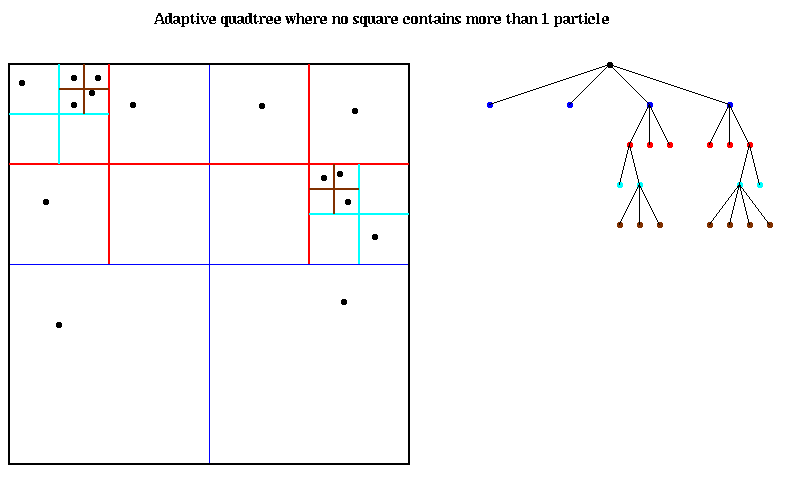
\includegraphics[width=0.9\textwidth]{graphics/bh/Quadtree2.png}
  \label{fig:bh-Quadtree2}
  \caption{Adaptive quadtree where no square contains more than 1 particle}
\end{figure}

\Level 0 {The Barnes-Hut Algorithm}
\label{sec:bh-barnes-hut}

At a high level, here is the Barnes-Hut algorithm:

\begin{enumerate}
\item  Build the Quadtree
\item  For each subsquare in the quadtree, compute the center of mass and total
mass for all the particles it contains. 
\item  For each particle, traverse the tree to compute the force on it.
\end{enumerate}

The core of the algorithm is computing the force on each particle. For that we use the
idea in the first figure above, namely that if the ratio:

\begin{verbatim}
D                      size of box
-  =  -----------------------------------------------
r     distance from particle to center of mass of box
\end{verbatim}

is small enough, then we can compute the force due to all the particles in the
box just by using the mass and center of mass of the particles in the box. We
will compare D/r to a user-supplied threshold theta (usually a little less than
1) to make this decision.

Thus, if D/r $<$ theta, we compute the gravitational force on the particle as if
all particles in the box were just one particle with mass being the total mass of
the particles in the box and the position being the center of mass of all the
particles in the box.




